Link prediction is the problem of forecasting connections between network nodes, even in cases of missing or undiscovered information. This is useful in various applications, such as recommending items for online purchase and predicting co-authorships in academic research networks. There are several different approaches are used to predict the link. In Neighbor-based approaches, a similarity score is computed between non-neighbor nodes. A high similarity score between the pair of nodes, indicates a higher likelihood of existence of a link between the two nodes \cite{gatadi2023lpcd, wang2014link}.

Link prediction is a paradigmatic problem in network science, which aims at estimating the existence likelihoods of non observed links, based on known topology \cite{zhou2021progresses}.

In this poster, we parallelize link prediction and present algorithmic techniques to significantly accelerate it. In addition, we use the parallel Dynamic Frontier Hybrid Louvain-LPA algorithm for community detection to further accelerate the dynamic community detection algorithm.

Lastly, we would like to emphasize that the soul of a network lies in its links instead of nodes; otherwise, we should pay more attention to set theory rather than graph theory \cite{zhou2021progresses}. Therefore, in network science, link prediction is a paradigmatic and fundamental problem with long attractivity and vitality \cite{zhou2021progresses}.

Early studies often compare a very few algorithms on several small networks according to one or two metrics \cite{zhou2021progresses}. Recent large-scale experiments \cite{mara2020benchmarking, ghasemian2020stacking, muscoloni2022adaptive, muscoloni2021short, zhou2021experimental} indicated that the above methodology may result in misleading conclusions. Future studies ought to implement systematic analyses involving more synthetic and real networks, benchmarks, state-of-the-art algorithms, and metrics \cite{zhou2021progresses}.

We expect a larger fraction of algorithms in the future studies will be designed for networks of particular types \cite{zhou2021progresses}.

Extensive experiments \cite{ghasemian2020stacking} show that no known link predictor performs best or worst across all inputs \cite{zhou2021progresses}.

Ghasemian et al. \cite{ghasemian2020stacking} argues that the ensemble models are usually superior to individual algorithms.

An individual algorithm could be highly cost-effective for its competitive performance and low complexity in time and space \cite{zhou2021progresses}.

In some real applications like friend recommendation, predictions with explanations are more acceptable \cite{barbieri2014follow}, which cannot be obtained by ensemble learning.


A network embedding algorithm will produce a function so that every node is represented by a low-dimensional vector \cite{cui2018survey}. Then, the existence likelihood of a non-observed link can be estimated by the inner product, the cosine similarity, the Euclidean distance, or the geometrical shortest path of the two learned vectors \cite{cui2018survey, cannistraci2013minimum}.

On the one hand, embedding is currently a very hot topic in network science and thought to be a promising method for link prediction. On the other hand, some very recent empirical studies \cite{muscoloni2022adaptive, mara2020benchmarking, ghasemian2020stacking} involving more than a thousand networks showed negative evidence that network embedding algorithms perform worse than some elaborately designed mechanistic algorithms.

Another notable embedding method is based on the hyperbolic network model \cite{krioukov2010hyperbolic, papadopoulos2012popularity}, where each node is represented by only two coordinates (i.e., d = 2) in a hyperbolic disk.

Matrix completion aims to reconstruct a target matrix, given a subset of known entries. Since links can be fully conveyed by the adjacency matrix A, it is natural to regard link prediction as a matrix completion task. Matrix factorization is a very popular method for matrix completion, which has already achieved great success in a closely related domain, the design of recommender systems \cite{koren2009matrix}.

Xian et al. \cite{xian2020netsre} suggested that the structural regularity corresponds to redundant information in the adjacency matrix, which can be characterized by a low-rank and sparse representation matrix. Sun et al. \cite{sun2020revealing} proposed a more direct method to measure such redundancy. Their train of thought is that a more predictable network contains more structural redundancy and thus can be compressed by a shorter binary string.

Koutra et al. \cite{koutra2015summarizing} found that the major part of a seemingly complicated real network can be represented by a few elemental substructures like cliques, stars, chains, bipartite cores, and so on. Inspired by this study, Xian et al. \cite{xian2020netsre} claimed that a network is more regular and thus more predictable if it can be well represented by a small number of subnetworks. 

Link prediction is essentially a compression problem [SAYS ME].


AUC is inadequate to evaluate the early retrieval performance which is critical in real applications \cite{zhou2021progresses}.

AUC will give misleadingly overhigh score to algorithms that can successfully rank many negatives in the bottom while this ability is less significant in imbalanced learning \cite{yang2015evaluating, lichtnwalter2012link}.

Performance evaluation metrics can be roughly divided into two categories: threshold-dependent metrics (e.g., fixed threshold accuracy) and threshold-independent metric (e.g., area under threshold curve) \cite{zhou2021progresses}. Precision and recall are the two most widely used metrics in the former category. Precision is defined as the ratio of relevant items selected to the number of items selected \cite{zhou2021progresses}. That is to say, if we take the top-$L$ links as the predicted ones; among which $L_r$ links are correctly predicted; then, the Precision equals $L_r/L$ \cite{zhou2021progresses}. Recall is defined as the ratio of relevant items selected to the total number of relevant items, say $L_r = |E^P|$ \cite{zhou2021progresses}. An obvious drawback of threshold-dependent metrics is that we generally do not have a reasonable way to determine the threshold, like the number of predicted links $L$ or the threshold score for the existence of links \cite{zhou2021progresses}. A widely adopted way is setting $L = |E^P|$, at which precision = recall \cite{lu2011link, liben2003link, zhou2021progresses}. Although $|E^P|$ is generally unknown, an experiential and reasonable setting is  $|E^P| = 0.1 |E|$ because $10\%$ of links in the probe set are usually enough for us to get statistical solid results while the removal of $10\%$ of links will probably not destroy the structural features of the target network \cite{lu2015toward}.

Consider a simple network $G(V, E)$, where $V$ and $E$ are sets of nodes and links, the directionalities and weights of links are ignored, and multiple links and self-connections are not allowed. We assume that there are some missing links or future links in the set of unobserved links $U - E$, where $U$ is the universal set containing all $|V|(|V|-1)/2$ potential links. The task of link prediction is to find out those missing or future links. To test the algorithm’s accuracy, the observed link, $E$, is divided into two parts: the training set $E^T$ is treated as known information, while the probe set $E^P$ is used for algorithm evaluation, and no information in $E^P$ is allowed to be used for prediction. The majority of known studies applied ‘‘random division’’, namely $E^P$ is randomly drawn from $E$ \cite{zhou2021progresses}.

Almost all obtained social network data is incomplete since only part of social information can be collected from social network platforms \cite{wang2014link}. Second, social networks are highly dynamic, which might lead the nodes and edges to appear or disappear in the future \cite{wang2014link}.

Link prediction has many important applications. First, it can be applied to recommender systems in information retrieval and e-commerce, which can help people to find new friends \cite{aiello2012friendship} and potential collaborators \cite{mori2012machine, recommendationpatent}, provide interesting items in online shopping \cite{akcora2011network}, recommend patent partners in enterprise social networks \cite{recommendationpatent} and cross-domain partners \cite{tang2012cross}, find experts or co-authors in academic social networks \cite{pavlov2007finding, wohlfarth2008semantic}, and predict cell phone contacts in large scale communication network \cite{raeder2011predictors}. Second, it also can be used to infer complete networks based on partial observed networks \cite{marchette2008predicting, kim2011network}, understand the evolution of networks better \cite{barabasi2002evolution, juszczyszyn2011link, bringmann2010learning, raymond2010fast}, and predict hyper-links in heterogeneous social networks \cite{zhu2002using}. Finally, the link prediction techniques can also be applied in bioinformatics and biology, for example, in health care and gene expression networks \cite{almansoori2012link}, predicting specialists who are more likely to receive future referrals, and finding protein-protein interactions. Even in other domains such as security related domain, it can be used to identify abnormal communications \cite{huang2009time}.

Link prediction aims to anticipate the probability of a future connection between two nodes in a given network based on their previous interactions and the network structure \cite{arrar2023comprehensive}.

It has applications in recommender systems - for a marketplace (to predict new items or products based on user’s preferences) \cite{su2020link, vahidi2021hybrid, su2019link}, social networks (to recommend new connections) \cite{abdolhosseini2020overlapping, daud2020applications}, in criminal networks through analysis of relationships and interactions between individuals to uncover criminal activities like drug trafficking or money laundering, and determine connections between those involved in such activities \cite{berlusconi2016link, lim2019hidden}, security domain (to assess trustworthiness of individuals) \cite{alnumay2019trust}, community detection (identify communities in a network) \cite{de2017community, esslimani2011densifying}, anomaly detection (for identifying missing links) \cite{huang2006link}, and in biological networks - protein-protein interactions (to predict new interactions and generate hypotheses) \cite{nasiri2021novel, cannistraci2013link}.

In recent years, the field of link prediction has witnessed a significant increase in research activities. Over the years, numerous methods have been developed for link prediction, encompassing similarity-based indices, dimensionality reduction based methods, machine learning techniques, and more \cite{arrar2023comprehensive}.

A large number of existing research work on link prediction focus on solving the problem of small networks. However, we are interested in addressing the problem for large networks. Instead of the AUC metric, we focus on precision-recall (which are ~same).




\subsection{Our Contributions}

This technical report proposes an approach for significantly improving the performance of existing local/neighbor-based link prediction techniques, both in terms of runtime and precision.

GVE-Leiden\footnote{https://github.com/puzzlef/neighborhood-link-prediction-openmp}, an optimized parallel implementation of the Leiden algorithm for community detection on shared memory multicores. On a machine with two 16-core Intel Xeon Gold 6226R processors, GVE-Leiden achieves a processing rate of $352 M$ edges/s on a $3.8 B$ edge graph, and outperforms the original Leiden implementation, igraph Leiden, and NetworKit Leiden by $373\times$, $86\times$, and $7.2\times$ respectively, while identifying communities of the same quality as the first two implementations, and $26\%$ higher quality than NetworKit. Compared to GVE-Louvain, our parallel Louvain implementation, GVE-Leiden achieves an $11$-fold reduction in internally-disconnected communities, with only a $36\%$ increase in computation time. With doubling of threads, GVE-Leiden exhibits an average performance scaling of $1.6\times$.\ignore{This makes GVE-Leiden an attractive choice for high-quality community detection on massive graphs.}




%% - Use --- for a dash.
%% - Use ``camera-ready'' for quotes.
%% - Use {\itshape very} or \textit{very} for italicized text.
%% - Use \verb|acmart| or {\verb|acmart|} for mono-spaced text.
%% - Use \url{https://capitalizemytitle.com/} for URLs.
%% - Use {\bfseries Do not modify this document.} for important boldface details.
%% - Use \ref{fig:name} for referencing.

%% For a block of pre-formatted text: 
% \begin{verbatim}
%   \renewcommand{\shortauthors}{McCartney, et al.}
% \end{verbatim}

%% For a list of items:
% \begin{itemize}
% \item the ``ACM Reference Format'' text on the first page.
% \item the ``rights management'' text on the first page.
% \item the conference information in the page header(s).
% \end{itemize}

%% For a table:
% \begin{table}
%   \caption{Frequency of Special Characters}
%   \label{tab:freq}
%   \begin{tabular}{ccl}
%     \toprule
%     Non-English or Math&Frequency&Comments\\
%     \midrule
%     \O & 1 in 1,000& For Swedish names\\
%     $\pi$ & 1 in 5& Common in math\\
%     \$ & 4 in 5 & Used in business\\
%     $\Psi^2_1$ & 1 in 40,000& Unexplained usage\\
%   \bottomrule
% \end{tabular}
% \end{table}

%% For a full-width table:
% \begin{table*}
%   \caption{Some Typical Commands}
%   \label{tab:commands}
%   \begin{tabular}{ccl}
%     \toprule
%     Command &A Number & Comments\\
%     \midrule
%     \texttt{{\char'134}author} & 100& Author \\
%     \texttt{{\char'134}table}& 300 & For tables\\
%     \texttt{{\char'134}table*}& 400& For wider tables\\
%     \bottomrule
%   \end{tabular}
% \end{table*}


%% For inline math:
% \begin{math}
%   \lim_{n\rightarrow \infty}x=0
% \end{math},

%% For a numbered equation:
% \begin{equation}
%   \lim_{n\rightarrow \infty}x=0
% \end{equation}

%% For an unnumbered equation:
% \begin{displaymath}
%   \sum_{i=0}^{\infty} x + 1
% \end{displaymath}

%% For a figure:
% \begin{figure}[h]
%   \centering
%   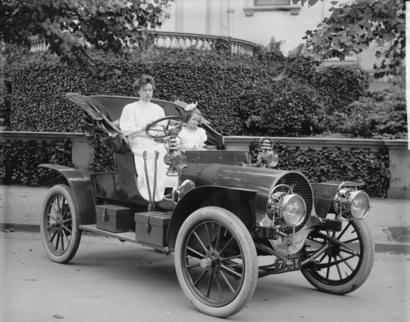
\includegraphics[width=\linewidth]{inc/sample-franklin}
%   \caption{1907 Franklin Model D roadster. Photograph by Harris \&
%     Ewing, Inc. [Public domain], via Wikimedia
%     Commons. (\url{https://goo.gl/VLCRBB}).}
%   \Description{A woman and a girl in white dresses sit in an open car.}
% \end{figure}

%% For a teaser figure.
% \begin{teaserfigure}
%   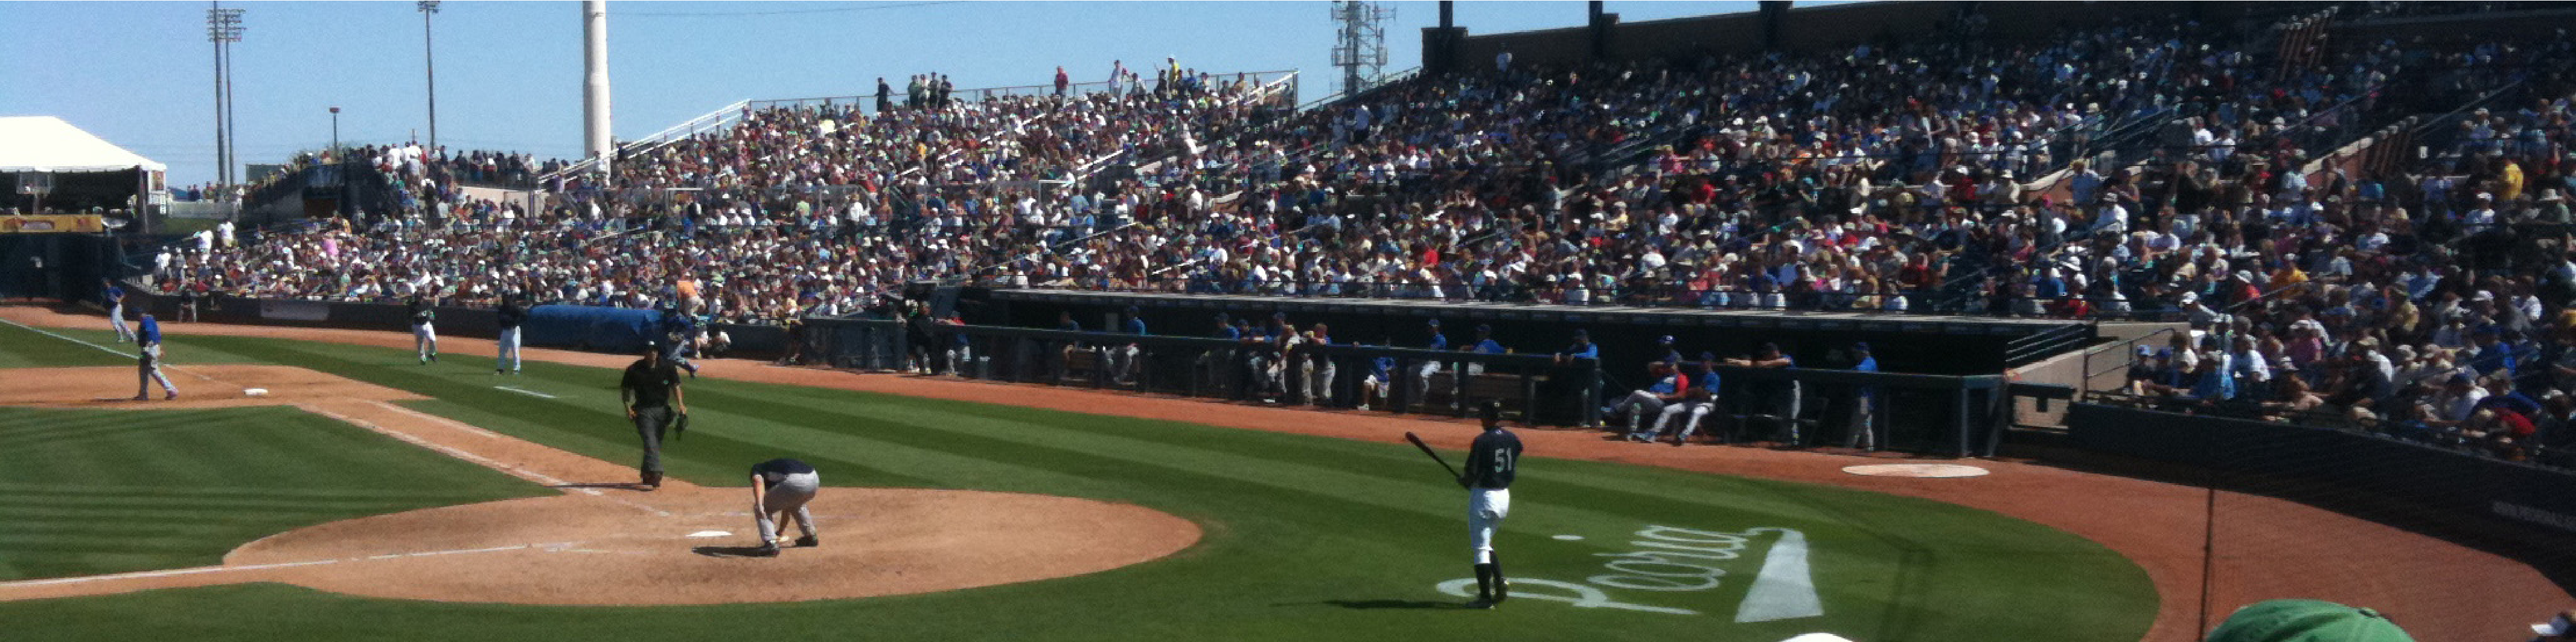
\includegraphics[width=\textwidth]{sampleteaser}
%   \caption{figure caption}
%   \Description{figure description}
% \end{teaserfigure}
